\documentclass[a5paper,twoside]{article}
\usepackage[T2A]{fontenc}
\usepackage[cp1251]{inputenc}
\usepackage[russian]{babel}
\usepackage[amsmath]{}
\usepackage{cleveref}
%\usepackage[dvips]{color}
%\usepackage[pdftex]{}
\usepackage{latexsym, eucal, bm, color, amsfonts, amssymb,amsmath, epsfig, a4wide}
\usepackage{indentfirst}
\usepackage{hyperref, cite}
%\usepackage{layout}
%\usepackage{nccboxes}

\usepackage{listings}
\lstloadlanguages{C, bash, Gnuplot}
\lstset{numbers=left, frame=single, breaklines=true, breakatwhitespace=true, title=\lstname, tabsize=2}

\newtheorem{theorem}{�������}[section]
\newtheorem{lemma}{�����}
\newtheorem{corollary}{���������}
\newtheorem{definition}{�����������}
\newtheorem{property}{��������}
\newtheorem{example}{������}
\newtheorem{remark}{���������}
\newtheorem{proposition}{�����������}
\newtheorem{hypothesis}{��������}
\newtheorem{exersize}{����������}


\pagestyle {plain}

\hoffset=-10.4mm \voffset=-12.4mm \oddsidemargin=5mm \evensidemargin=0mm \topmargin=0mm \headheight=0mm \headsep=0mm
\textheight=174mm \textwidth=113mm

%\binoppenalty=10000 \relpenalty=10000

\makeatletter
%\renewcommand{\section}{\@startsection{section}{1}{0pt}{-3.5ex plus -1ex minus -.2ex}{2.3ex plus.2ex}{\center\normalfont\Large\bfseries}}
%\renewcommand{\subsection}{\@startsection{subsection}{2}{0pt}{-2.5ex plus -1ex minus -.2ex}{1.3ex plus.2ex}{\center\normalfont\large\bfseries}}

\selectlanguage{russian}

% ��������������� ������. ���� ���-�� �������,
% ����������� ������������ ����!
% ����������� \��,\��, \����� �������� ��� ���������� ������ �� ��������
% � ���� ����������. ��� ��������� �� ������ �� ������ � ������ ���������.
%        /�. ����������/
%\expandafter\ifx\csname russcorr.sty\endcsname\relax
%        \expandafter\def\csname russcorr.sty\endcsname{}
%\else\endinput\fi
%\def\@versiondate{6 ���� 1994}
%\typeout{��� - russcorr.sty <\@versiondate>}
%\typeout{������������� �� ������: �.�.���������, serge@schcorr.msk.su}
%
% ��� ������ �������� ������� ��������� �������
%\message{Correcting math definitions,}
%\let\labelenumiii\relax  % ??? ����� ���?
%\let\theenumiii\relax    % � ���??
%
% ������ ��������� �������� ������������������ � ������ �������
% ��� - ��� ������������� � NFSS
\expandafter\ifx\csname selectfont\endcsname\relax
% ��� ������ FSS:
\def \tg {\mathop{\rm tg}\nolimits}
\def \ctg {\mathop{\rm ctg}\nolimits}
\def \cosec {\mathop{\rm cosec}\nolimits}
\def \arctg {\mathop{\rm arctg}\nolimits}
\def \arcctg {\mathop{\rm arcctg}\nolimits}
\def \sh {\mathop{\rm sh}\nolimits}
\def \ch {\mathop{\rm ch}\nolimits}
\def \th {\mathop{\rm th}\nolimits}
\def \cth {\mathop{\rm cth}\nolimits}
\def \rect {\mathop{\rm rect}\nolimits}
\else % ��� NFSS:
\def \tg {\mathop{\operator@font tg}\nolimits}
\def \ctg {\mathop{\operator@font ctg}\nolimits}
\def \cosec {\mathop{\operator@font cosec}\nolimits}
\def \arctg {\mathop{\operator@font arctg}\nolimits}
\def \arcctg {\mathop{\operator@font arcctg}\nolimits}
\def \sh {\mathop{\operator@font sh}\nolimits}
\def \ch {\mathop{\operator@font ch}\nolimits}
\def \th {\mathop{\operator@font th}\nolimits}
\def \cth {\mathop{\operator@font cth}\nolimits}
\def \rect {\mathop{\operator@font rect}\nolimits}
\def \sign {\mathop{\operator@font sign}\nolimits}
\fi
\let\eps\varepsilon
\let\vphi\varphi
% ��������� �������� �����
%
\@ifundefined{chapter}{\def\@mainstyle{A}}{% ��� �� ������
\@ifundefined{abstractname}{\def\@mainstyle{B}}% ��� �� report
{\def\@mainstyle{R}}}
%
% ������ ��������� ���������
%
\message{heading names,}
\def\contentsname{����������}
\def\figurename{���.}
\def\partname{�����}     % �������, ��� �� ������ ������� �����
\def\chaptername{�����}  % ������ ������
\def\listfigurename{������ ��������}
\def\listtablename{������ ������}
\def\refname{����������}
\def\bibname{����������}
\def\indexname{���������� ���������}
\def\tablename{�������}
\def\abstractname{���������}
%
%
% ������ �������� �������� � �������.
% ����� ������ ����� ����� ������ ����� ����� � ��������.
%
\message{headings,}
\def\chapter{\clearpage % ��� �������� ������ - ������ \cleardoublepage
   \thispagestyle{plain}%
   \global\@topnum\z@
   \@afterindenttrue % ����� ��������� (���� \@afterindentfalse)
   \secdef\@chapter\@schapter}
%
% ����� � ������ ����� ����� ������ ������, ��������� � ������������
% ����� � ��������, �� ��� ���� �� �������� �����������
% �������� � ���������: ��� ����� ���� � ���� �������� \def'��
% �������� �� ����� ���� ���������� ��������� ������� \@startsection
% (��������, {-3.5ex plus-1ex minus-.2ex} ��� \section ).
%
% ������� ��������, ��� ��� ����������� �� ������� �� ����� � �����,
% ����� ��� �������� � art12.sty � ���� �������� ������� ������!
%
\def\section{\@startsection {section}{1}{\z@}{2.5ex plus 1ex minus
    .2ex}{1.5ex plus.2ex}{\reset@font\Large\center\bf}}
\def\subsection{\@startsection{subsection}{2}{\z@}{2.0 ex plus 1 ex
    minus .2ex}{1.5ex plus.2ex}{\reset@font\large\center\bf}}
\def\subsubsection{\@startsection{subsubsection}{3}{\z@}{3.25ex plus
    1ex minus.2ex}{1.5ex plus.2ex}{\reset@font\normalsize\center\bf}}
%
% � ��������, ����� ��������� ������� � ������ ������,
% ������� ��� ���, ����� � ���������� ����� ������ ��������� �����.
% ��������: 4.3. ���-��� � ������
%
% ����� ��������� ����������� �������� � ���������,
% ������ ������� \aftersectionseparator � �.�. (��. ����)
% � ��������� �� ������. ����� ��������� � ��������, ���� ��������������
% �� �� \relax ��� {}
% ����� ���������� �� � ��� ���-������, ���� ����� �������� � ������.
%
% �������, ���, ���� ������ ������� ���-������ ���������
%  \def\thesection{\arabic{chapter}.\arabic{section}.} ,
% �� ��������� �������� � \label � \ref .
%
\def\@aftersepkern{\kern-.5em}
\def\postchapter{.}
\def\postsection{.\@aftersepkern}
\def\postsubsection{.\@aftersepkern}
\def\postsubsubsection{.\@aftersepkern}
\def\postparagraph{.\@aftersepkern}
\def\postsubparagraph{.\@aftersepkern}
\def\presection{}
\def\presubsection{}
\def\presubsubsection{}
\def\preparagraph{}
\def\presubparagraph{}
%
%  ��������� � ���������� ����� ����� �������...
%
\def\@sect#1#2#3#4#5#6[#7]#8{\ifnum #2>\c@secnumdepth
     \let\@svsec\@empty\else
     \refstepcounter{#1}\edef\@svsec{%
     \csname pre#1\endcsname % ������� ������
     \csname the#1\endcsname
     \csname post#1\endcsname % ������� ������
\hskip 1em}\fi
     \@tempskipa #5\relax
      \ifdim \@tempskipa>\z@
        \begingroup #6\relax
          \@hangfrom{\hskip #3\relax\@svsec
                   }{\interlinepenalty \@M \ignorespaces#8\par}%
% ������� � ���������� ������ \ignorespaces
% ����� � ����� ����� ������� - ������ ������ ��������, ������������,
% ���� �������� sectioning-������� ���������� � �������.
        \endgroup
       \csname #1mark\endcsname{\protect\ignorespaces #7}\addcontentsline
% ������� ��� token'� ����� #7
         {toc}{#1}{\ifnum #2>\c@secnumdepth \else
                      \protect\numberline{\csname the#1\endcsname
                     \csname post#1\endcsname % ������� ������
}\fi \protect\ignorespaces #7}\else
% ������� ��� token'� ����� #7
        \def\@svsechd{#6\hskip #3\relax  %% \relax added 2 May 90
                   \@svsec #8\csname #1mark\endcsname
                      {\protect\ignorespaces #7}\addcontentsline
% ������� ��� token'� ����� #7
                           {toc}{#1}{\ifnum #2>\c@secnumdepth \else
                             \protect\numberline{\csname the#1\endcsname
                          \csname post#1\endcsname % ������� ������
}\fi \protect\ignorespaces #7}}\fi
% ������� ��� token'� ����� #7
     \@xsect{#5}}
\def\@ssect#1#2#3#4#5{\@tempskipa #3\relax
   \ifdim \@tempskipa>\z@
     \begingroup #4\@hangfrom{\hskip #1}{\interlinepenalty \@M
\ignorespaces #5\par}\endgroup % ������� \ignorespaces ����� #5
   \else \def\@svsechd{#4\hskip #1\relax
\ignorespaces #5}\fi % ������� \ignorespaces ����� #5
    \@xsect{#3}}
% ����� ������� ���� ���� ����� ����� �����:
%
\def\@makechapterhead#1{%
  \vspace*{50\p@}%
  {\parindent \z@\raggedright
    \ifnum \c@secnumdepth >\m@ne
     \huge\bf \@chapapp{} \thechapter\postchapter % ��������� \postchapter
    \par
    \vskip 20\p@ \fi
    \Huge \bf
    \ignorespaces #1\par % ������� \ignorespaces
    \nobreak
    \vskip 40\p@
  }}
\def\@makeschapterhead#1{%
  \vspace*{50\p@}%
  {\parindent \z@ \raggedright
    \Huge \bf
    \ignorespaces #1\par % ������� \ignorespaces
    \nobreak
    \vskip 40\p@
  }}
%
% ������� ���, ���� � ���������� ����� ��� � ����� ������� ����...
%
\def\@chapter[#1]#2{\ifnum \c@secnumdepth >\m@ne
        \refstepcounter{chapter}%
        \typeout{\@chapapp\space\thechapter.}%
        \addcontentsline{toc}{chapter}{\protect
        \numberline{\thechapter
              \postchapter % ������� ������
}%
\protect\ignorespaces #1}\else % ������� ��� token'� ����� #1
      \addcontentsline{toc}{chapter}{\protect\ignorespaces#1}\fi
% � ���������� ������� ��������� ��� token'� ����� #1
   \chaptermark{\protect\ignorespaces #1}%
   \addtocontents{lof}%
       {\protect\addvspace{10\p@}} % Adds between-chapter space
   \addtocontents{lot}%
       {\protect\addvspace{10\p@}} % to lists of figs & tables.
   \if@twocolumn                   % Tests for two-column mode.
           \@topnewpage[\@makechapterhead{#2}]%
     \else \@makechapterhead{#2}%
           \@afterheading          % Routine called after chapter and
     \fi}                          % section heading.
%
% ������ ��������� ������� � �������� � ��������
%
%---------Modified by BaSSiLL--------------

\newcommand{\captionwidth}{\textwidth}
\newcommand{\captionlinestretch}{1.0}
\newcommand{\captionfontsize}{\normalsize}

\message{captions,}
\long\def\@makecaption#1#2{%
%-------- The following line was replaced by the line after it:
%  \vskip 10\p@
  \vskip 5\p@
  \setbox\@tempboxa\hbox{\captionfontsize #1. #2}% �������� ��������� �� �����...
  \ifdim \wd\@tempboxa >\captionwidth
  {
    \renewcommand{\baselinestretch}{\captionlinestretch}
    \selectfont
    \centerline{
        \begin{tabular}{p{\captionwidth}}
            \unhbox\@tempboxa \\
        \end{tabular}
    }\par
  }
  \else \centerline{\box\@tempboxa}\fi

%-------- The following line was added:
  \vskip 5\p@
%------------------------------------------
} \long\def\@caption#1[#2]#3{\par\addcontentsline{\csname
  ext@#1\endcsname}{#1}{\protect\numberline{\csname
  the#1\endcsname.}{\ignorespaces #2}}\begingroup
    \@parboxrestore
    \normalsize
    \@makecaption{\csname fnum@#1\endcsname}{\ignorespaces #3}\par
  \endgroup}

%
% ��������� �������� - ��������� ����� ����� ������� "������".
% �� ����� ��������� \afterthmseparator � ��������������
% ��� ������. ��� �������� � ��������� - ��������������
% ��� �� \relax
%
\message{theorems,}
\def\afterthmseparator{.}
\def\@begintheorem#1#2{\trivlist \item[\hskip \labelsep{\bf
#1\ #2\unskip\afterthmseparator}]\it} % ������� 2 token'� ����� #2
\def\@opargbegintheorem#1#2#3{\trivlist
      \item[\hskip \labelsep{\bf
#1\ #2\ (#3)\afterthmseparator}]\it} % ������� token ����� (#3)
%
% �������� ����������� (�� �� ����� ����� ������).
\message{running heads,}
\if A\@mainstyle % ����� - article (��������� ".\@aftersepkern" ����� ������)
  \if@twoside
   \def\ps@headings{\let\@mkboth\markboth
    \def\@oddfoot{}\def\@evenfoot{}%       No feet.
    \def\@evenhead{\rm \thepage\hfil \sl \leftmark}%        Left heading.
    \def\@oddhead{{\sl \rightmark}\hfil \rm\thepage}% Right heading.
    \def\sectionmark##1{\markboth {\uppercase{\ifnum \c@secnumdepth >\z@
      \thesection\postsection \hskip 1em\relax \fi ##1}}{}}%
    \def\subsectionmark##1{\markright {\ifnum \c@secnumdepth >\@ne
            \thesubsection\postsubsection \hskip 1em\relax \fi ##1}}}
  \else
   \def\ps@headings{\let\@mkboth\markboth
    \def\@oddfoot{}\def\@evenfoot{}%     No feet.
    \def\@oddhead{{\sl \rightmark}\hfil \rm\thepage}% Heading.
    \def\sectionmark##1{\markright {\uppercase{\ifnum \c@secnumdepth >\z@
      \thesection\postsection \hskip 1em\relax \fi ##1}}}}
  \fi
\else\if R\@mainstyle % �����=report. ��� ������� ����� ����� �������� �� ����.
  \if@twoside
  \def\ps@headings{\let\@mkboth\markboth
   \def\@oddfoot{}\def\@evenfoot{}%       No feet.
   \def\@evenhead{\rm \thepage\hfil \sl \leftmark}%        Left heading.
   \def\@oddhead{{\sl \rightmark}\hfil \rm\thepage}% Right heading.
   \def\chaptermark##1{\markboth {\uppercase{\ifnum \c@secnumdepth >\m@ne
        \@chapapp\ \thechapter. \fi ##1}}{}}%
   \def\sectionmark##1{\markright {\uppercase{\ifnum \c@secnumdepth >\z@
     \thesection. \fi ##1}}}}
  \else
  \def\ps@headings{\let\@mkboth\markboth
  \def\@oddfoot{}\def\@evenfoot{}%     No feet.
  \def\@oddhead{{\sl \rightmark}\hfil \rm\thepage}% Heading.
  \def\chaptermark##1{\markright {\uppercase{\ifnum \c@secnumdepth >\m@ne
    \@chapapp\ \thechapter. \fi ##1}}}}
  \fi
\else % �����=book (��� ������� ����� ����� �������� �� ����)
\def\ps@headings{\let\@mkboth\markboth
 \def\@oddfoot{}\def\@evenfoot{}%       No feet.
 \def\@evenhead{\rm \thepage\hfil \sl \leftmark}%        Left heading.
 \def\@oddhead{{\sl \rightmark}\hfil \rm\thepage}% Right heading.
 \def\chaptermark##1{\markboth {\uppercase{\ifnum \c@secnumdepth >\m@ne
      \@chapapp\ \thechapter. \fi ##1}}{}}%
 \def\sectionmark##1{\markright {\uppercase{\ifnum \c@secnumdepth >\z@
   \thesection. \fi ##1}}}}
\fi\fi
%
% ��������� ������� \appendix : ��������� �������� �������,
% � �� ����������.
\message{appendix,} \if A\@mainstyle
\def\appendix{\par
  \setcounter{section}{0}%
  \setcounter{subsection}{0}%
  \def\thesection{\Ralph{section}}}
\else
\def\appendix{\par
  \setcounter{chapter}{0}%
  \setcounter{section}{0}%
  \def\@chapapp{\appendixname}%
  \def\thechapter{\Ralph{chapter}}}
\fi

% ��������� ��� ���� feature: \cleardoublepage ������ ��
% ������ �������� ����������, ���������� �� ����������� �������.
% ������� ���, ����� ����� �� ����...
\message{\string\output,}
\def\cleardoublepage{\clearpage\if@twoside \ifodd\c@page\else
   {\null\ps@empty % ������� \ps@empty (� ������ ������� \hbox{} �� \null )
\newpage}\if@twocolumn\hbox{}\newpage\fi\fi\fi}

%
% ������ "������������" ��������� enumerate:
%\def\labelenumi{\theenumi)}      % ����� ����� ������ ��� ������;
\def\theenumii{\ralph{enumii}}   % ����� �� ������ ������ ��� �������,
\def\labelenumii{\theenumii)}    % � �� ��������� �����
\def\p@enumii{\theenumi}         % � ��� ��� \ref
\def\labelenumiii{{\bf--}}       % � �� ������� ������ ����� ����� ���� ����,
\let\theenumiii\relax            % � ��������� ������ �� ���� �� �����
\def\p@enumiii{\theenumi\theenumii}
%
% � ��� �������� ���������� ������ enumerate ���� � ����� ...
%
\def\enumerate{\ifnum \@enumdepth >2% ���� 3, � �� 2
\@toodeep\else
      \advance\@enumdepth \@ne
      \edef\@enumctr{enum\romannumeral\the\@enumdepth}\list
      {\csname label\@enumctr\endcsname}{\usecounter
        {\@enumctr}\def\makelabel##1{\hss\llap{##1}}}\fi}
%
% ������ ��������� ��������� rlist
% ��� �������� �������, � �������
% \item'� ���������� �������� �������
% (��������� ��� rlist, ���������� ��� rlist[u])
%
\@definecounter{rlistctr}
\newif\if@rlistsnested\@rlistsnestedfalse % ��������� ������� ����� ��
% ���������, �� Lamport � ����������� ��������� ��� ������
\def\rlist{\@ifnextchar[{\@rlist}{\@rlist[l]}}
\def\@rlist[#1]{\if u#1\def\@tempa{R}\else\def\@tempa{r}\fi
                \if@rlistsnested\@toodeep\else
                \@rlistsnestedtrue
                \edef\therlistctr{\expandafter\noexpand\csname
                                @\@tempa alph\endcsname\noexpand\c@rlistctr}%
                \list{\labelrlist}{\usecounter
                   {rlistctr}}\fi}
\let\endrlist\endlist
\def\labelrlist{\therlistctr)}
%
% � ������ ��������� �������-"�����"
%
\message{quotes,}
%
% !!!! ������ � �� ������� ��������� !!!! ��� ������ �� german.sty
\def\set@low@box#1{\setbox\tw@\hbox{,}\setbox\z@\hbox{#1}\dimen\z@\ht\z@
     \advance\dimen\z@ -\ht\tw@
     \setbox\z@\hbox{\lower\dimen\z@ \box\z@}\ht\z@\ht\tw@ \dp\z@\dp\tw@ }
%    (this lowers the german left quotes to the same level as the comma.)
\def\@glqq{{\ifhmode \edef\@SF{\spacefactor\the\spacefactor}\else
     \let\@SF\empty \fi \leavevmode
     \set@low@box{''}\box\z@\kern-.04em\@allowhyphens\@SF\relax}}
\def\glqq{\protect\@glqq}
\def\@grqq{\ifhmode \edef\@SF{\spacefactor\the\spacefactor}\else
     \let\@SF\empty \fi \kern-.07em``\kern.07em\@SF\relax}
\def\grqq{\protect\@grqq}
\def\@glq{{\ifhmode \edef\@SF{\spacefactor\the\spacefactor}\else
     \let\@SF\empty \fi \leavevmode
     \set@low@box{'}\box\z@\kern-.04em\@allowhyphens\@SF\relax}}
\def\glq{\protect\@glq}
\def\@grq{\kern-.07em`\kern.07em}
\def\grq{\protect\@grq}
% !!!!
%
% � ������ ��������� �������-"������" � ���� ������.
% ��� ������ ������ ����� ����, ��� � ������ ���������
% ��������������� �������.
%
% ��� ��������� ����������� --- �� ������,
% ���� ������� ����� �� ��� � �� ������ �������...
\expandafter\ifx\csname flqq\endcsname\relax\chardef\flqq=192 \fi \expandafter\ifx\csname frqq\endcsname\relax\chardef\frqq=193
\fi \expandafter\ifx\csname No\endcsname\relax\chardef\No=194 \fi
% � ��� -- ���������� �����������:
\expandafter\ifx\csname documentclass\endcsname\relax \expandafter\ifx\csname ��\endcsname\relax\chardef\��=192 \fi
\expandafter\ifx\csname ��\endcsname\relax\chardef\��=193 \fi \expandafter\ifx\csname �����\endcsname\relax\chardef\�����=194
\fi \fi
%
% �� ���������� ����������:
\expandafter\ifx\csname documentclass\endcsname\relax
\def\�������{\number\day\space
                \ifcase\month\or
                 ������\or �������\or �����\or ������\or ���\or
                 ����\or ����\or �������\or ��������\or �������\or
                 ������\or �������\fi\space\number\year}
\fi
%\message{...finished.}
\endinput



\hyphenation {��-����-��-���� ��-��-��� ���-����-����� ��-���-��-����}

\begin{document}

\newcommand  {\op      } [1]     { \bm{#1}           }
\renewcommand{\vec     } [1]     { \bm{#1}           }
\newcommand  {\vr      }         { \vec{r}           }
\newcommand  {\vR      }         { \vec{R}           }
\newcommand  {\paren   } [1]     { \left( #1 \right) }
\def          \fun       _#1(#2) { #1 \paren{#2}     }
\newcommand  {\inv     } [1]     { \frac{1}{#1}      }
\def          \pdsqr     _#1_#2  { \frac{\partial^2}{\partial #2^2}#1 }
\newcommand  {\dsr   } { \fun_{\Delta s^2}(\vr) }
\newcommand  {\rmR   } { \vr - \vR }
\newcommand  {\rmrz  } { \vr - \vec{r}_0 }
\newcommand  {\rmrw  } { \vr - \tilde{\vec{r}} }
\newcommand  {\Rmrw  } { \vR - \tilde{\vec{r}} }
\newcommand  {\armR  } { \left| \rmR  \right| }
\newcommand  {\armrw } { \left| \rmrw \right| }
\newcommand  {\aRmrw } { \left| \Rmrw \right| }
\newcommand  {\armrz } { \left| \rmrz \right| }
\renewcommand{\L     } { \fun_L(\vR,t|\vr) }

\pagestyle{plain}

\sloppy \fontsize {10dd}{12dd} \selectfont

\begin {titlepage}
\begin{center}
%------------------------------------------------------------------------------------
{\footnotesize ������������ ����������� � ����� ���������� ���������

%\vspace{1em}

 ���������� ������-����������� ��������

(��������������� �����������)

}


\vspace{6mm}

{\itshape ������� �����������

}

\vspace{23mm}

{\large \bfseries{���������� �������-������������������ ���� ��� ��������� ����������� ��������� ��������}}

\vspace{20mm}

{\large ������-������������ �������

}

\end{center}
\vspace{30mm}
\begin{flushright}
����������� \emph{�.�.~�������}
\end{flushright}

\vspace{15mm}
\begin{center}
������ \\ ���� \\ 2013
\end{center}
\end{titlepage}
%------------------------------------------------------------------------------------
\thispagestyle{empty}
\begin{flushleft}
��� 519.63
\end{flushleft}

\begin{center}
��������� \\ {\small �������� ������-�������������� ���� \emph{�.�.~������}}
\end{center}

{\bfseries ���������� �������-������������������ ���� ��� ��������� ����������� ��������� ��������}: ������-������������ �������
/ ����. �.�.~�������. -- �.:~����,~2013. -- 22~�.

\vspace{10mm}

������ ��������� ���������� ��������� ��������-������������������ ������� ��� ������� ��������� ����������� ��������� ��������, ������� ��������� � �������
�������� ������ ������ � ��������, ������� �������� � ������������ ������� �������� ����.
��������������� ��� ���������, ��������� �����������, � ���� �������� �� ���������� �������������� ���������� �� ����� ��.

\vspace{74mm}








{\footnotesize %\scriptsize

\hspace{13.6em} \copyright\  �������~�.�., 2013

\hspace{13.6em} \copyright\  ����������� ��������������� ����������

\hspace{15.3em}��������������� ����������

\hspace{15.3em}������� ����������������� �����������

\hspace{15.3em}<<���������� ������-����������� ��������

\hspace{15.3em}(��������������� �����������)>>, 2013

}\newpage
%\nopagenumbers
%\newpage
%------------------------------------------------------------------------------------


\vspace{100mm}

\fussy \tableofcontents \sloppy

\clearpage

\begin{center}
\Large { \textbf {�������-������������������ ������ ��� ���������� ������� ����������� ��������� ��������� ��������}}
\end{center}
\rule[5pt]{\textwidth}{0.5pt} \vspace {-8mm}

\section*{��������}
\addcontentsline{toc}{section}{��������}

��������������� ������� ��������� ���������� ������ �������������� ������� ��������� ���������� ��������� [1. ������� �.�. ��������� ������ ������� ��������� � ������ ���������������� ���� // ������������ ������������������ ������. �.VII-1. �.2. �.: ����-�, 2008, �.141-174], [2. ������ �.�., ������� �.�. ��������� ������������ ��������� ������������ ����� �������� �������������� ������� ���� �������-������������������ ������� // ������ �������������� ���������� � �������������� ������, 1984. - �. 24, � 5. - �. 722 - 739.], [2. ������� �.�., ������ �.�., ������ �.�. ��������� ������������� ������������ ���������� �������-������������������ ������� // ������ �������������� ���������� � �������������� ������, 2013. � �. 53, � 10. � �. 1709 � 1720.], [������ �.�., ������ �.�. ������������� ����� 3D �������� �� ���������������������� �������������� �������� // �������������� �������������, 2014. - �. 26, � 1. - �. 83 - 95.].
� ��� ���������: ������ ������� ��������, �������-�������� ����, ���������� �������������.
� ���������, ������������� ����� ���������� �����, ������������, ��� ��������� ��������, ��� � ���������� � ���������� ���������, �� ����� �������������� �������.
����� �������, ������ ������� �������� �������� ������������ � ���������� ����� ��������� ������� ��� ������� ��������������� ������ ���������.

����� �� �������� � ���������� ��������� ������� ������� ��������������� ������ ��������� �������� ����� ����������� �� ���������������� ����������, �������, ��������� � ��������������� ������� ����������, ��������� ������ ������ � ����������������� ������� ������ �������� ���������� ��������� ��������.
������ ������ ��������� �������� ���������� �������� ��������� ������� ��� ��� �������.
��������������� ����� ������, ���������� �� �������-������������������ ������ � ������������ ������� ������� ���������� �� ��������� �������.
������� ��� ��������� ������� ��������� ������� ������������� �����: ���������� ����������������� ������� [2. Rusanov V.V. Calculation of intersection of non-steady shock waves with obstacles // J. Comput. Math. Phys. USSR. 1961. Vol. 1. P. 267-279] � ���������� ��������� ��������� ��� ���������������� ���������� [3. Courant, Richard and Lax, Peter On nonlinear partial differential equations with two independent variables // Communications on Pure and Applied Mathematics, 1949. Vol. 2. P255-273].
���������� ������ ���������� ��������� ���� �� ����� ��, ���������� ������ ��� ��������������� ������.

\subsection*{���������� �������� ��������� ��������}

���������� ���������� �������� ��������� ��������:
\begin{equation}
\label{eq_advection}
u_t + \lambda u_x  = 0.
\end{equation}

��� $u(x,t)$ - ������� �������, ��������, ������������ ���������� ������ � ��������, $\lambda$ - �������� ��������.
����� ������ ����������
\begin{equation}
\label{eq_ksi}
\xi = x - \lambda t
\end{equation}

� ����� ������ ������� ��������� \ref{eq_advection} � ���� $u(\xi)$.
������ ������������ ����� ���������, ��� \ref{eq_advection} ������������ � ���������.
����� �������, ���� ����������� ��� ���������������� ������� ������� $t^n$ � $t^n+\tau$, ����� �������� ��������� ���������:
\begin{equation}
\label{eq_grid_feature}
u(x_m, t_n+\tau) = u(x_m-\lambda\tau, t_n).
\end{equation}

�� ���� ������� �������� �������� ����� ������������ �������-������������������ ��������� ������� [4. ��������� �.�., ������� �.�. �������-������������������ ��������� ������ // �����, 1988. 287 �.].
��� ���������� �������� ����� ��������� � ������������� $\lambda\geq0$, ��������� ��������� �� ������ �������������� ������������ ���� ������ $\lambda$ �� $-\lambda$ � ��������� ������� �� ��������������� �� ������������ �����.

\subsection*{���������� �������� ��������� ������� ��������}

���������� ������ � ��������������� ���� �������� ����� ��������� � ���� � ���������� ����������.
����� �������, ��� ������������ ��������� ��������������� ������� ��������� ������� ����, ���������� $\rho_0$ � ��������� $P(\rho_0)$.
������������ ��������� �������� �������� $p(x, t)$ � �������� $u(x, t)$, ��� ����� �������� ������������ ����������� ��������.
���� ������ ����������� $K_0=\rho_0 P'(\rho_0)$, �� ������������ ��������, ������������ � �����, ����� ���� ������� �������� �������� ���������������� ���������: 
\begin{equation}
\label{eq_acoustic}
\left[ \begin{array}{c} p \\ u \end{array} \right]_t
+
\left[ \begin{array}{cc} 0 & K_0 \\ \frac{1}{\rho_0} & 0 \end{array} \right]
\left[ \begin{array}{c} p \\ u \end{array} \right]_x
= 0.
\end{equation}

����������� �������� ������� ������ ������� $\lambda_{1,2}=\pm c_0$, ��� $c_0=\sqrt{P'(\rho_0)}$.
������� $S$, ������������ �� ����������� ��������, � �������� � ��� $S^{-1}$ ����� ��� ��������������:
\begin{equation}
\label{eq_acoustic_eigmat}
S=\left[ \begin{array}{cc} -Z_0 & Z_0 \\ 1 & 1 \end{array} \right],
S^{-1}=\frac{1}{2Z_0}\left[ \begin{array}{cc} -1 & Z_0 \\ 1 & Z_0 \end{array} \right],
\end{equation}
��� $Z_0=\rho_0c_0$.

����� �������, ������� \ref{eq_acoustic} ����� ���� ���������� � ����:
\begin{equation}
\label{eq_acoustic_simply}
\left[ \begin{array}{c} p \\ u \end{array} \right]_t
+
S\left[ \begin{array}{cc} -c_0 & 0 \\ 0 & c_0 \end{array} \right]S^{-1}
\left[ \begin{array}{c} p \\ u \end{array} \right]_x
= 0.
\end{equation}

�������� ��� ����� \ref{eq_acoustic_simply} �� $S^{-1}$ ����� � ����� ������ ����������
\begin{equation}
\label{eq_acoustic_change}
\left[ \begin{array}{c} w_1 \\ w_2 \end{array} \right]=S^{-1} \left[ \begin{array}{c} p \\ u \end{array} \right]
=\frac{1}{2Z_0}
\left[ \begin{array}{c} -p + Z_0u \\ p + Z_0u \end{array} \right].
\end{equation}
������� ��������� ������� ���������:
\begin{equation}
\label{eq_acoustic_rim}
\left[ \begin{array}{c} w_1 \\ w_2 \end{array} \right]_t
+
\left[ \begin{array}{cc} -c_0 & 0 \\ 0 & c_0 \end{array} \right]
\left[ \begin{array}{c} w_1 \\ w_2 \end{array} \right]_x
= 0.
\end{equation}

����� �������, ��� ������� ������ � ��������������� ���� ����� ��������� � ���� ���������� ������ ��� ����������� ��������� �������� � ���������� $w_1, w_2$ � ������� ������� � ���������� $p$ � $u$.

\subsection*{���������� �������� ��������� ������� �����}

���������� ������ � ��������������� ���� �������� ����� ��������� � ������� ����� � ���������� ����������.
���������� ������ � ���������������� ���������� � ���� ����������� ������� ����� ������������� �� ����������� ��������.
� ��� ��������� ���������� $\sigma_{xx}(x, t)$ � �������� ����� $u(x, t)$.
������������� ����� �����������: $\lambda$ � $\mu$ - ������� ��������� ����, $\rho$ - ��������� �����.
������������ ��������, ������������ � �����, ����� ���� ������� �������� �������� ���������������� ���������: 
\begin{equation}
\label{eq_elastic}
\left[ \begin{array}{c} \sigma_{xx} \\ u \end{array} \right]_t
+
\left[ \begin{array}{cc} 0 & -(\lambda + 2\mu) \\ -\frac{1}{\rho} & 0 \end{array} \right]
\left[ \begin{array}{c} \sigma_{xx} \\ u \end{array} \right]_x
= 0.
\end{equation}

����������� �������� ������� ������ ������� $\lambda_{1,2}=\pm c_p$, ��� $c_p=\sqrt{\frac{\lambda+2\mu}{\rho}}$.
������� $S$, ������������ �� ����������� ��������, � �������� � ��� $S^{-1}$ ����� ��� ��������������:
\begin{equation}
\label{eq_acoustic_eigmat}
S=\left[ \begin{array}{cc} Z & -Z \\ 1 & 1 \end{array} \right],
S^{-1}=\frac{1}{2Z}\left[ \begin{array}{cc} 1 & Z \\ -1 & Z \end{array} \right],
\end{equation}
��� $Z=\rho c_p$.

���������� \ref{eq_acoustic_change} ��������� ������ ����������
\begin{equation}
\label{eq_elastic_change}
\left[ \begin{array}{c} w_1 \\ w_2 \end{array} \right]=S^{-1} \left[ \begin{array}{c} \sigma_{xx} \\ u \end{array} \right]
=\frac{1}{2Z}
\left[ \begin{array}{c} \sigma_{xx} + Zu \\ -\sigma_{xx} + Zu \end{array} \right]
\end{equation}

�������� ������� ��������� \ref{eq_elastic} ����� ������������� � ����:
\begin{equation}
\label{eq_elastic_rim}
\left[ \begin{array}{c} w_1 \\ w_2 \end{array} \right]_t
+
\left[ \begin{array}{cc} -c_p & 0 \\ 0 & c_p \end{array} \right]
\left[ \begin{array}{c} w_1 \\ w_2 \end{array} \right]_x
= 0.
\end{equation}

����� �������, ��� ������� ������ � ��������������� ������� ���� ����� ��������� � ����� ���������� ������ ��� ����������� ��������� �������� � ���������� $w_1, w_2$ � ������� ������� � ���������� $\sigma_{xx}$ � $u$.

\section {�������-������������������ ����� �� ����������� �������}

\subsection {���������� � ������}

�������� ��������� \ref{eq_grid_feature} ���������� ����� ����������� ��������������� �������� ������� ������� $u(x,t)$ � ������������ ����� ��������� �������, ����� ��� ��� ��������� ������� � �������� �������� � ������������� ����� ��������� �����.
��� ������� ������ ������ ������������� ���������� ������������ ������� ��������� �������� �������.
�������, ��� ��� ��������������� ����� ����� ���������� � ������ ����, �.�. �� ���� $n+1$ ����� �������������� ������ ���� ����� ������� $x^{n+1}_m$.

���������� ������������ �� ������������ ������ ���. \ref{stencil_2_2}.
�� ��� ����� ��������� ������� ������ ������� �� ��������� ������� � ����� $x^n_m$ � $x^n_{m-1}$.

\begin{figure}[h]
  \center
  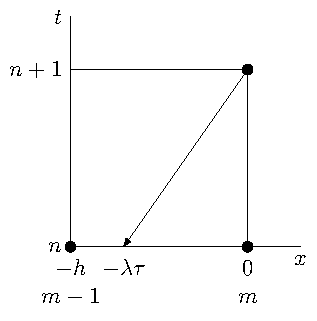
\includegraphics[scale=1.0]{pictures/stencil_2_2.pdf}
  \caption{������������ �� ������������ ������, ������������ ��� ���������� ����� ������� �������}
\label{stencil_2_2}
\end{figure}

� ����� ���� ������� ������� ������� ���������� � ����:
\begin{equation}
\label{eq_polynom_1}
F_1(x) = a_1x + b_1.
\end{equation}

������������ $a_1$ � $b_1$ ����� ���� ������� �� ������� ����������� �������� $F_1(x)$ ����� �������� �������, �������� � ����� �������:
\begin{eqnarray*}
\label{eq_polynom_1_params} 
a_1 = \frac{u^n_m - u^n_{m-1}}{h}, \\
b_1 = u^n_m.
\end{eqnarray*}

���������� �� � ��������� \ref{eq_polynom_1} � ��������� ����������� \ref{eq_grid_feature}, �������:
\begin{equation}
\label{eq_polynom_1_schema} 
u^{n+1}_m = u^n_m - \frac{\lambda\tau}{h}(u^n_m - u^n_{m-1}).
\end{equation}

�������� ������� � ���������� ����� �������� ��������� ������� ������������� ����� �� ������������ �������� ���������� ��������� �������.

�������� ������ � ������������� �����������, ������� ����� $x^n_{m+1}$.
�� ��� ����� ���� �������� ������� ������ �������, � ����� ���� ������������ ������������:
\begin{equation}
\label{eq_polynom_2} 
F_2(x) = a_2x^2 + b_2x + c_2.
\end{equation}

������������ $a_2$, $b_2$ � $c_2$ ����� ���� ������� �� ������� ����������� �������� $F_2(x)$ ����� �������� �������, �������� � ����� �������:
\begin{eqnarray*}
\label{eq_polynom_2_params}
a_2 = \frac{u^n_{m+1} - 2u^n_m + u^n_{m-1}}{2h^2}, \\
b_2 = \frac{u^n_{m+1} - u^n_{m-1}}{2h}, \\
c_2 = u^n_m.
\end{eqnarray*}

���������� �� � ��������� \ref{eq_polynom_2} � ��������� ����������� \ref{eq_grid_feature}, �������:
\begin{equation}
\label{eq_polynom_2_schema} 
u^{n+1}_m = u^n_m - \frac{\lambda\tau}{2h}(u^n_{m+1} - u^n_{m-1}) + \frac{\lambda^2\tau^2}{2h^2}(u^n_{m+1}
- 2u^n_m + u^n_{m-1}).
\end{equation}

��� ����������� ��������� ������� ����� �������� ������, ������� � ���� ����� $x_{m-2}$.
�� ��� ����� ���� �������� ������� ������� �������, � ����� ���� ������������ ������������:
\begin{equation}
\label{eq_polynom_3} 
F_3(x) = a_3x^3 + b_3x^2 + c_3x + d_3.
\end{equation}

������������ $a_3$, $b_3$, $c_3$ � $d_3$ ����� ���� ������� �� ������� ����������� �������� $F_3(x)$ ����� �������� �������, �������� � ����� �������:
\begin{eqnarray*}
\label{eq_polynom_3_params}
a_3 = \frac{u^n_{m+1} + 3u^n_{m-1} -3 u^n_m - u^n_{m-2}}{6h^3}, \\
b_3 = \frac{u^n_{m+1} - 2u^n_m + u^n_{m-1}}{2h^2}, \\
c_3 = \frac{2u^n_{m+1} + 3u^n_m - 6u^n_{m-1} + u^n_{m-2}}{6h}, \\
d_3 = u^n_m.
\end{eqnarray*}

���������� �� � ��������� \ref{eq_polynom_3} � ��������� ����������� \ref{eq_grid_feature}, �������:
\begin{eqnarray}
\label{eq_polynom_3_schema} 
u^{n+1}_m = u^n_m - \frac{\lambda\tau}{6h}(2u^n_{m+1} + 3u^n_m -6u^n_{m-1} + u^n_{m-2}) + \nonumber\\
+ \frac{\lambda^2\tau^2}{2h^2}(u^n_{m+1} - 2u^n_m + u^n_{m-1}) - \nonumber\\
- \frac{\lambda^3\tau^3}{6h^3}(u^n_{m+1} + 3u^n_{m-1} - 3u^n_m - u^n_{m-2}).
\end{eqnarray}

��� ����������� ��������� ������� ����� �������� ������, ������� � ���� ����� $x_{m+2}$.
�� ��� ����� ���� �������� ������� �������� �������, � ����� ���� ������������ ������������:
\begin{equation}
\label{eq_polynom_4} 
F_4(x) = a_4x^4 + b_4x^3 + c_4x^2 + d_4x + e_4.
\end{equation}

������������ $a_4$, $b_4$, $c_4$, $d_4$ � $e_4$ ����� ���� ������� �� ������� ����������� �������� $F_4(x)$ ����� �������� �������, �������� � ����� �������:
\begin{eqnarray*}
\label{eq_polynom_4_params}
a_4 = \frac{6u^n_m - 4u^n_{m+1} - 4u^n_{m-1} + u^n_{m+2} + u^n_{m-2}}{24h^4}, \\
b_4 = \frac{2u^n_{m-1} - 2u^n_{m+1} + u^n_{m+2} - u^n_{m-2}}{12h^3}, \\
c_4 = \frac{16u^n_{m+1} - 30u^n_m + 16u^n_{m-1} - u^n_{m+2} - u^n_{m-2}}{24h^2}, \\
d_4 = \frac{8u^n_{m+1} - 8u^n_{m-1} - u^n_{m+2} + u^n_{m-2}}{12h}, \\
e_4 = u^n_m.
\end{eqnarray*}

���������� �� � ��������� \ref{eq_polynom_4} � ��������� ����������� \ref{eq_grid_feature}, �������:
\begin{eqnarray}
\label{eq_polynom_4_schema}
u^{n+1}_m = u^n_m - \frac{\lambda\tau}{12h}(8u^n_{m+1} - 8u^n_{m-1} - u^n_{m+2} + u^n_{m-2}) + \nonumber\\
+ \frac{\lambda^2\tau^2}{24h^2}(16u^n_{m+1} - 30u^n_m + 16u^n_{m-1} - u^n_{m+2} - u^n_{m-2}) - \nonumber\\
- \frac{\lambda^3\tau^3}{12h^3}(2u^n_{m-1} - 2u^n_{m+1} + u^n_{m+2} - u^n_{m-2}) + \nonumber\\
+ \frac{\lambda^4\tau^4}{24h^4}(6u^n_m - 4u^n_{m+1} - 4u^n_{m-1} + u^n_{m+2} + u^n_{m-2}).
\end{eqnarray}

\textbf{$\blacktriangle$ ����������������� �������}

\begin {enumerate}
\item{��������� ����� ���������� �������� ������������� (������� � 5-��) ���� ���������� ��������� ������� ������� $x^n_{m-3}, x^n_{m+3}, x^n_{m-4}, x^n_{m+4}$, � �.�. ��������������.
�������, ��� ��������� �� ��� ����� �� �������� ��������� ������������ [5. ������ �.�. ������ �� �������������� ����������: ������� ������� / �.�. ������, �.�. �������. - �.: ��������-����������� �������������� ����������; �����. ����������� ������, 2006. - 523 �.].
���������, ����� ����� ���������� �������� ��� �� ������������ ����������.}
\item{��� ���� ������� �����, ��� ������ $\lambda<0$ ����� ������� ������� ����� ���� �������� ������� ������� ����� � ������������ ����� � �������� �� $x^n_{m-1}$ � $x^n_{m+1}$.
���������, ��� ����� ����������� ��������� �����, � ������� ����������� ����� ����� ���� ����� ������.
���������� ������ - �������� ������ ������ � �������� �� ��������� ������ � �������� (������������� ��� �������������) �����������.}
\item{��������, ��� �������-������������������ ����� ��� ������������� ��������� ������� ������� ��������� �� ������ �����-��������� [5. Lax, P.D., Wendroff, B. System of conservation laws / P.D. Lax, B. Wendroff // Comm. Pure and Appl. Math. � 1960. � Vol. 13, No. 2. � P. 217 � 237.].}
\item{��������, ��� �������-������������������ ����� ��� ������������� ��������� �������� ������� ��������� �� ������ �������� [6. Rusanov, V.V. Calculation of intersection of non-steady shock waves with obstacles / V.V. Rusanov // J. Comput. Math. Phys. USSR. � 1961. � Vol. 1. � P. 267-279].}
\end {enumerate}

\subsection {���������� �� ����� ��}

\lstset{language=C}

��������� �������������� ��������� ����� ���� ����������������� �� ����� ����� ����������������.
���������� ���������� ��������� ���� �� ����������� ������� ��� ������� ����������� ��������� ��������� �������� �� ����� ��.

��������� ���������� ����� ��������� ������� ������� � �������.
��� ����� �������, ��������, ����� ����� ���������� ������� �� ������ ���� ������������ � ������� ���������� ���� ������� ������������ ��� ��������� ������������ ����.
���������� ���� � ����������� ������� \textbf{advection.h}.

\lstinputlisting{./src/advection.h}

����������� $N$ ����� ���������� �����, �� ������� ����������� ��������� ������� $[-1, 1$], � ���������� �������� $U\_c$ � $U\_n$ �������� �������� ������� ������� �� ������� � ��������� ��������� ����, ��������������.
������� $initialize(void)$ ���������� ���������� ������� $U\_c$ ��������� ��������, $singleStep()$ - ��������� ���� ��� ��������� �����, ������� � ����� �� ���� ����� �����.
������� $interpolatedValue(double\;*u)$ �������� ������������ �� ������ ������� � ���������� �������� �������� � ����� $x_0=-\lambda\tau$, $debugPrint()$ - ������� ��������� �������� ���������� ���� � ����������� ���� �� ����������� ����� ������, $debugGnuplot()$ - ��������� � ���� ��� ������������ ���������� �������� � ��������� Gnuplot.
�� ���������� ��������� � ����� \textbf{advection.c}.

\lstinputlisting{./src/advection.c}

������������ �����������: $l=\lambda$, $h$ - ��� �����, $tau$ - ��� �� �������, $k=\frac{l*tau}{h}$, $M$ - ����� ����� �� �������.
����������� ��� ���� ��������� �������, ������������ � ����������� �� ������ ����������:
\begin{enumerate}
\item{ROUGH\_INITIAL - ��������� ������������� ��������� �������, �������� � ������ �������.}
\item{SMOOTH\_INITIAL - ������� ������� $sin^4(\pi x)$, �������� �� ���� �������.}
\end{enumerate}

��� ���������� ���������� ��������� ������������ �� ��������� ������� �������� ����������� ����.
� ������ $int\;stencil$ � ����������� �� ������ ���������� ������������ �������� (� ��������) ����� ������������ ������������, ��������������� ������������� �������.
������������� ���������� ������ $double\;stencil\_values$, � ������� ����� ���������� ������� ���� ����������� �������� �� ������� $U\_c$, ��������������� ������ �������.
��� ���� ����������� ����������� ��������� �������, �.�. ������ �� �������� ������� ���� ������������� ������� ����� ����.

��� ���������� ��������� ������������ ������ \textbf{build.sh}.

\lstset{language=bash}

\lstinputlisting{./src/build.sh}

������������� ������� ������� �� ������� �������, ����������� �������� $debugGnuplot(void)$, ����� ���� ���������������, ��������, �������� \textbf{plot.plot}.

\lstset{language=Gnuplot}

\lstinputlisting{./src/plot.plot}

�� ���. \ref{wide_stencil_cmp} ��������� ��������� ��������� �������, ���������� ������� �� ����������� ��������.
� �������� ���������� ������� ������������� ��������� ������������� �������, �������� � ������ ��������� �������.
������������ ������������� ������� ������� ����� ������ ������� �������.

\begin{figure}[h]
  \center
  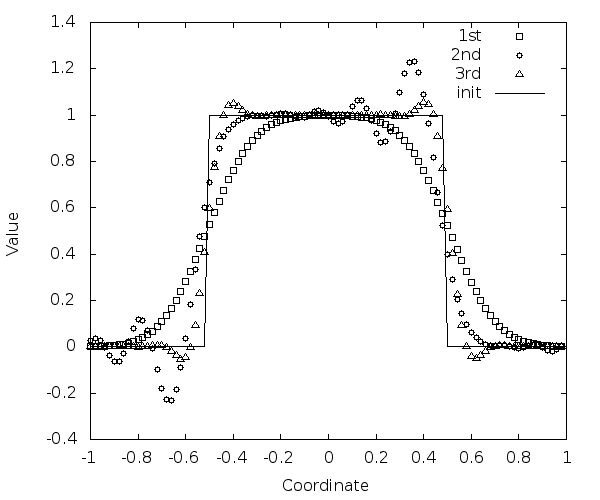
\includegraphics[scale=0.6]{src/images/wide/fig_wide_stencil_cmp_rough.png}
  \caption{��������� ���� 1-3 �������� �� ����������� ��������}
\label{wide_stencil_cmp}
\end{figure}

\textbf{$\blacktriangle$ ����������������� �������}

\begin {enumerate}
\item{����������� ��������� \textbf{Advection} ��� ���������� ����� 4-�� ������� �������� ������, ���������� � ���������� �����.
��������� ��������� ����� �� ������� � ��������� ��������.}
\item{����������� ��������� \textbf{Advection} ��� ���������� ���� ����������� �������, ���������� �� ���������� ��������� �������.
��������� ��������� ���� �� ������� � ��������� ��������.}
\end {enumerate}

\clearpage

\section{������� ��������� ��������}

\subsection {������� � ���������� ������}

���������� ������ � ��������������� ���� �������� ����� ��������� � ���� � ���������� ����������.
����� �������, ��� ����������� ��������� ��������������� ������� ��������� ������� ����, ���������� $\rho_0$ � ��������� $P(\rho_0)$.
������������ ��������� �������� �������� $p(x, t)$ � �������� $u(x, t)$, ��� ����� �������� ������������ ����������� ��������.
���� ������ ����������� $K_0=\rho_0 P'(\rho_0)$, �� ������������ ��������, ������������ � �����, ����� ���� ������� �������� �������� ���������������� ���������: 
\begin{equation}
\label{eq_acoustic}
\left[ \begin{array}{c} p \\ u \end{array} \right]_t
+
\left[ \begin{array}{cc} 0 & K_0 \\ \frac{1}{\rho_0} & 0 \end{array} \right]
\left[ \begin{array}{c} p \\ u \end{array} \right]_x
= 0.
\end{equation}

����������� �������� ������� ������ ������� $\lambda_{1,2}=\pm c_0$, ��� $c_0=\sqrt{P'(\rho_0)}$.
������� $S$, ������������ �� ����������� ��������, � �������� � ��� $S^{-1}$ ����� ���:
\begin{equation}
\label{eq_acoustic_eigmat}
S=\left[ \begin{array}{cc} -Z_0 & Z_0 \\ 1 & 1 \end{array} \right],
S^{-1}=\frac{1}{2Z_0}\left[ \begin{array}{cc} -1 & Z_0 \\ 1 & Z_0 \end{array} \right],
\end{equation}
��� $Z_0=\rho_0c_0$.

����� �������, ������� (\ref{eq_acoustic}) ����� ���� ���������� � ����
\begin{equation}
\label{eq_acoustic_simply}
\left[ \begin{array}{c} p \\ u \end{array} \right]_t
+
S\left[ \begin{array}{cc} -c_0 & 0 \\ 0 & c_0 \end{array} \right]S^{-1}
\left[ \begin{array}{c} p \\ u \end{array} \right]_x
= 0.
\end{equation}

�������� ��� ����� (\ref{eq_acoustic_simply}) �� $S^{-1}$ ����� � ����� ������ ����������
\begin{equation}
\label{eq_acoustic_change}
\left[ \begin{array}{c} w_1 \\ w_2 \end{array} \right]=S^{-1} \left[ \begin{array}{c} p \\ u \end{array} \right]
=\frac{1}{2Z_0}
\left[ \begin{array}{c} -p + Z_0u \\ p + Z_0u \end{array} \right],
\end{equation}
������� ��������� ������� ���������:
\begin{equation}
\label{eq_acoustic_rim}
\left[ \begin{array}{c} w_1 \\ w_2 \end{array} \right]_t
+
\left[ \begin{array}{cc} -c_0 & 0 \\ 0 & c_0 \end{array} \right]
\left[ \begin{array}{c} w_1 \\ w_2 \end{array} \right]_x
= 0.
\end{equation}

����� �������, ��� ������� ������ � ��������������� ���� ����� ��������� � ���� ���������� ������ ��� ����������� ��������� �������� � ���������� $w_1, w_2$ � ������� ������� � ���������� $p$ � $u$.

\subsection {���������� ���������� ����}

���������� ������� ��������� �������� (\ref{eq_acoustic_rim}).
����� �������������� ������� ������� � ���������������� ���������� ���������:
\begin{equation}
\label{eq_extended_rim}
\begin{cases}
\nu_1(x,t)=\frac{\partial w_1}{\partial x}(x,t), \\
\nu_2(x,t)=\frac{\partial w_2}{\partial x}(x,t), \\
\nu_1(x,0)=\frac{\partial w_1}{\partial x}(x,0), \\
\nu_2(x,0)=\frac{\partial w_2}{\partial x}(x,0).
\end{cases}
\end{equation}

������� (\ref{eq_acoustic_rim}) � (\ref{eq_extended_rim}) ������ �������� ��� ����������� ������������ ������� ��� ��������� �������� $w_1$ � $w_2$, ������� ����� ������, ��������� ���������� ����� ���������� �����.
������ (\ref{eq_grid_feature}), ����� ��������, ���
\begin{eqnarray*}
\label{eq_grid_feature_w1w2}
w_1(x_m, t_n + \tau) = w_1(x_m + c_0\tau, t_n), \\
w_2(x_m, t_n + \tau) = w_2(x_m - c_0\tau, t_n).
\end{eqnarray*}

����� �������, ����������� ������ ��� ������� ������������ ������� �������� � ���� ������ ����� ${x^{n+1}_m, x^n_m, x^n_{m-1}, x^n_{m+1}}$ [10].
���� ������� �������� (\ref{eq_acoustic_eigmat}), ����� ���������� �������� ����������� ������ �� ������� ���� �� ������� ����� ���������� ������:
\begin{eqnarray*}
\label{w1w2_n_pu}
w^n_{1,m} = \frac{1}{2Z_0}(-p^n_m + Z_0u^n_m), \\
w^n_{2,m} = \frac{1}{2Z_0}(p^n_m + Z_0u^n_m).
\end{eqnarray*}

��� ������� ������ �� ������������ ������ ����� ��������������� ���������� ������ �������� ������� ��������.
����� ��� $w_2$ ����� �����
\begin{eqnarray*}
\label{eq_interpolated_w2}
w^n_2(x) = a_2x^3 + b_2x^2 + c_2x + d_2, \\
\nu^n_2(x) = 3a_2x^2 + 2b_2x + c_2, \\
a_2 = \frac{\nu^n_{2, m}+\nu^n_{2, m-1}}{h^2} - 2\frac{w^n_{2,m}-w^n_{2,m-1}}{h^3}, \\
b_2 = \frac{2\nu^n_{2, m}+\nu^n_{2, m-1}}{h} - 3\frac{w^n_{2,m}-w^n_{2,m-1}}{h^2}, \\
c_2 = \nu^n_{2,m}, \\
d_2 = w^n_{2,m}, \\
w^{n+1}_{2,m}=w^n_2(x_m - c_0\tau), \\
\nu^{n+1}_{2,m}=\nu^n_2(x_m - c_0\tau).
\end{eqnarray*}

� ��� $w_1$ ����� ����� (\textit{��������������� �������� ���������� ��������������}):
\begin{eqnarray*}
\label{eq_interpolated_w1}
w^n_1(x) = a_1x^3 + b_1x^2 + c_1x + d_1, \\
\nu^n_1(x) = 3a_1^x2 + 2b_1x + c_1, \\
a_1 = \frac{\nu^n_{1, m+1}+\nu^n_{1, m}}{h^2} - 2\frac{w^n_{1,m+1}-w^n_{1,m}}{h^3}, \\
b_1 = -\frac{\nu^n_{1, m+1}+2\nu^n_{1, m}}{h} + 3\frac{w^n_{1,m+1}-w^n_{1,m}}{h^2}, \\
c_1 = \nu^n_{1,m}, \\
d_1 = w^n_{1,m}, \\
w^{n+1}_{1,m}=w^n_1(x_m + c_0\tau), \\
\nu^{n+1}_{1,m}=\nu^n_1(x_m + c_0\tau).
\end{eqnarray*}

���� ������� �������� (\ref{eq_acoustic_eigmat}), ����� ���������� �������� ���������� ������ ����� �������� ����������� ������ �� ��������� ���� �� �������:
\begin{eqnarray*}
\label{pu_n_w1w2}
p^{n+1}_m = Z_0(-w^{n+1}_{1,m} + w^{n+1}_{2,m}), \\
u^{n+1}_m = w^{n+1}_{1,m} + w^{n+1}_{2,m}.
\end{eqnarray*}

\textbf{$\blacktriangle$ ����������������� �������}

\begin {enumerate}
\item{��������� ���������� ����� ������ ������� �������� ��� ������� ��������� ��������.
������� ����� � ���� ������ ������ � � ������?
���������� �������� ������������� ���������� ����, ����������� �� ������� ����� �����. � ���, ��-������, ����������� �� ����������?}
\item{��������� ������ ���������� ����������������� ������� ��� ��������� �������� �����, ��������� ����� � 1 �� 5 ������� ������������.}
\end {enumerate}

\subsection {���������� �� ����� C}

\lstset{language=C}

������ ��������������� ���������� � ����������� ������, �.�. ������� �� �������� � �������� � ���, � ����� �������� ������� �� ���������������.
����� ����, ��� ����� ������������� ����� ����������� �� ���������� � ���� ���������� �������� �� ���������� ��������, ���� ��������������� ������� ��������� ������� $interpolatedValue$, $interpolatedDValue$, $fillStencilValues$ � $singleStep$.
��������� ������� ��������� � ����� \textbf{acoustic\_ext.h}, � �� ����������~-- � ����� \textbf{acoustic\_ext.c}.
��� ������ ��������� ����� ���� ����������� ������ \textbf{build\_ac\_ext.sh}.

\lstinputlisting{./src/build_ac_ext.sh}

\lstinputlisting{./src/acoustic_ext.h}

\lstinputlisting{./src/acoustic_ext.c}

��� ������ ���������� ���������� �������� �� ������ ���� ������������ ������� ��������� ������� �� �������� �����������, ����������� ��� ���������� ���������� �����.

\textbf{$\blacktriangle$ ����������������� �������}

\begin {enumerate}
\item{������������� ��������� \textbf{Acoustic\_ext}, ������� ����� �������� �� ���������� ($p$, $u$) � ���������� ($w_1$, $w_2$) � �������.}
\item{������������� ��������� \textbf{Acoustic\_ext} ���, ����� ������ ������ ��������� ���������� ������������� �������� ��� ������� �������� ������� � � �����������.}
\item{������������� ��������� \textbf{Acoustic\_ext} ���, ����� ������ ������������� � ��������� ���������� ������������� �������� ��� $w_1$ � $w_2$.
\textit{���������}: �������� ����������� ������ ��� $w_1$.}
\item{����������� ��������� \textbf{Acoustic\_ext} ��� ���������� ����� 5-�� �������.
��������� ��������� ����� �� ������� � ��������� ��������.}
\item{*������������ ��������� ��� ������� ������� ��������� �������� � ��������� � ��������� �������.
\textit{���������}: ����������� ������ ����������� �� ������������.}
\end {enumerate}

\clearpage

\section*{����������}
\addcontentsline{toc}{section}{����������}
1.\,\emph{��������\,�.�.}\ \  ����������������\ \  ����\ \  �\ \  �������.\ \  --\,M.: ������ �����, 2007.

2.\,\emph{��������\,�.�.} ���������������� ���� � �������. --\,M.: ������ �����, 2007.

3.\,\emph{�����\,�.} �������� �����. ������������� ������ � ������������\ \  ����������~~/~~���.\ \  �\ \  ����.\ \  --\,M.:\ \  ������������\ \   ��� <<�������>>, 2008.


\clearpage
%-------------------------------------------------------------------------------------------
%\headsep = 20mm
\thispagestyle{empty}
\begin{center}

������� �������

\vspace{25mm}

{\large ���������� �������-������������������ ���� ��� ��������� ����������� ��������� �������� }

\vspace{6mm}

������������ ��������

\vspace{6mm}

�� ����� \emph{�����������}

\vspace{6mm}

{\large �����������} \textbf{�������}~�������~��������

%\vspace{14mm}
\vspace{38,5mm}

\small {�������� \emph{�.�.~������}. ��������� \emph{�.�.~������}}

\small {������������ ������� \emph{�.�.~�������}}

\end{center}

%\vspace{2mm}

\begin{flushleft}

{\small

��������� � ������ 24.01.2013. ������ 60$\times$84 $^{1}/_{16}$.

���. ���. �. 3,25. ��.-���.�. 3,0. ����� 120 ���. �����~�17.

%\vspace{24.5mm}

\rule[2pt]{\textwidth}{0.2pt}

����������� ��������������� ���������� ��������������� \\
���������� ������� ����������������� ����������� "<���������� \\
������-����������� ��������(��������������� �����������)">\\
141700, ���������� ���., �. ������������, ������������ ���., 9\\
E-mail: rio@mail.mipt.ru

\rule[2pt]{\textwidth}{0.2pt}
����� ����������� ���������� "<������-��������">\\
141700, ���������� ���., �. ������������, ������������ ���., 9\\
E-mail: polygraph@mipt.ru

}

\end{flushleft}


\end{document}
